\documentclass[11pt,a4paper]{article}
\usepackage[margin=2.4cm]{geometry}
\usepackage{amsmath,amssymb}
\usepackage{graphicx}
\usepackage{listings}
\usepackage{xcolor}
\usepackage[colorlinks=true,linkcolor=blue!50!black,citecolor=blue!50!black,urlcolor=blue!50!black]{hyperref}
\usepackage{natbib}
\lstset{basicstyle=\ttfamily\scriptsize,columns=fullflexible,breaklines=true,
        frame=single,rulecolor=\color{gray!50},keywordstyle=\color{blue!60!black},
        commentstyle=\color{green!40!black},language=Python,showstringspaces=false}
\newcommand{\dd}{\mathrm{d}}
\newcommand{\rc}{r_c}
\newcommand{\Rb}{R_b}
\newcommand{\Rmax}{R_{\max}}

\title{The disc that the seed's own angular momentum would make\\[4pt]
\large A companion note to \emph{From a primordial fluctuation to an idealised rotation curve}}
\author{B. R. Parodi}
\date{23 October 2026}

\begin{document}
\maketitle

\begin{abstract}
In the seed of the main paper every shell rotates rigidly with the
specific angular momentum it receives by turnaround, $j\propto M$. If the
gas of each mass element keeps its own angular momentum and settles on a
circular orbit in the final rotation curve, the disc that forms is fixed
completely by the seed. We derive its surface density in closed form for
a flat rotation curve, compute it numerically for the P18 curve with its
core, and compare it with an exponential disc and with the relation of
\citet{Mo1998} used in the main paper. The seed disc is close to
exponential between one and four scale lengths, but it has twice the
exponential mass inside half a scale length and a sharp edge at
$\Rmax=3\sqrt2\lambda GM/v\simeq4.3\,R_d$. Its scale length is 1.06 to
1.4 times the Mo--Mao--White value, depending on how $R_d$ is defined for
a non-exponential disc, and it depends only weakly on the spin. None of
this changes the conclusions of the main paper; it lowers the inferred
retained fraction of angular momentum $f_j$ and leaves the failed spin
test as it is.
\end{abstract}

\section{Motivation}

The main paper tests the energy closure with discs: if the stellar disc
keeps a fraction $f_j$ of the seed's specific angular momentum, then
$R_d/\rc=f_j\lambda y/\sqrt2$ (its Sect.~6.5). This relation assumes an
exponential disc in a flat rotation curve, for which the specific angular
momentum is $j_d=2vR_d$ \citep{Fall1980,Mo1998}. But the seed carries
more information than its mean angular momentum: it fixes how the
angular momentum is \emph{distributed} over its mass. Under detailed
conservation, each mass element keeping its own $j$
\citep{Mestel1963,Fall1980}, this distribution fixes the disc. The
question of this note is whether the disc so obtained is exponential, and
how its scale length compares with the Mo--Mao--White value.

\section{Theory}

\subsection{Angular momentum of the seed}

As in the main paper we use units with $G=v=1$, where $v$ is the flat
speed, and measure masses in units of the seed mass $M_{\rm tot}$. A shell
enclosing the mass $M$ turns around at $R_{\rm ta}=2GM/v^2$ and receives
by then, through tidal torques, the specific angular momentum
\begin{equation}
  j_{\rm sh}(M)=\sqrt2\,\lambda\,vR_{\rm ta}=2\sqrt2\,\lambda\,\frac{GM}{v},
  \label{eq:jsh}
\end{equation}
chosen so that the total angular momentum, $J=\int_0^Mj_{\rm sh}\,\dd M'=\sqrt2\lambda GM^2/v$,
returns the spin parameter of \citet{Peebles1969},
$\lambda=J|E|^{1/2}/(GM^{5/2})$ with $|E|=\tfrac12v^2M$, for every $M$.
Each shell rotates rigidly about a common axis $z$. A mass element at
polar angle $\theta$ has $j_z=\omega R^2\sin^2\theta$, and averaging
$\sin^2\theta$ over the sphere ($\langle\sin^2\theta\rangle=\tfrac23$)
gives $j_{\rm sh}=\tfrac23\omega R^2$; hence
\begin{equation}
  j_z=\tfrac32\,j_{\rm sh}(M)\,\sin^2\theta
     =3\sqrt2\,\lambda\,\frac{GM}{v}\,(1-\mu^2),\qquad \mu=\cos\theta .
  \label{eq:jz}
\end{equation}
Since the shells are equally spaced in $M$ and the mass of a shell is
spread uniformly in $\mu$, the seed is a population of mass elements
with $M/M_{\rm tot}$ and $\mu$ uniformly distributed in $[0,1]$. The
largest angular momentum, on the equator of the outermost shell, is
$j_{\max}=3\sqrt2\lambda GM_{\rm tot}/v$, and the mean is
$\langle j_z\rangle=j_{\max}\langle M/M_{\rm tot}\rangle\langle1-\mu^2\rangle
=j_{\max}\cdot\tfrac12\cdot\tfrac23=\sqrt2\lambda GM_{\rm tot}/v$, the
specific angular momentum of the seed.

\subsection{Detailed conservation and the disc}

Let a fraction of the matter be gas that keeps a fraction $f_j$ of its
own $j_z$ and settles on the circular orbit with that angular momentum in
the final rotation curve $v_c(R)$:
\begin{equation}
  R\,v_c(R)=f_j\,j_z .
  \label{eq:orbit}
\end{equation}
Then the distribution of $j_z$ over the mass becomes the distribution of
disc mass over radius. We take the gas to be a fixed fraction of every
mass element, so the disc mass $M_d$ is distributed as the seed's
$j_z$.

\paragraph{Flat rotation curve (analytic).} With $v_c=v$ the orbit
radius is $R=f_jj_z/v$, and with $S=R/\Rmax$,
\begin{equation}
  \Rmax=\frac{f_jj_{\max}}{v}=3\sqrt2\,f_j\lambda\,\frac{GM_{\rm tot}}{v^2},
  \qquad S=\frac{M}{M_{\rm tot}}\,(1-\mu^2).
\end{equation}
The disc mass inside $S$ is the fraction of the unit square
$(M/M_{\rm tot},\mu)$ where $(M/M_{\rm tot})(1-\mu^2)<S$. For
$1-\mu^2<S$, i.e.\ $\mu>\sqrt{1-S}$, every $M$ qualifies; otherwise only
$M/M_{\rm tot}<S/(1-\mu^2)$. Hence
\begin{equation}
  F(S)\equiv\frac{M_d(<R)}{M_d}
  =\bigl(1-\sqrt{1-S}\bigr)+\int_0^{\sqrt{1-S}}\frac{S\,\dd\mu}{1-\mu^2}
  =1-\sqrt{1-S}+S\,\operatorname{artanh}\sqrt{1-S},
  \label{eq:F}
\end{equation}
using $\int\dd\mu/(1-\mu^2)=\operatorname{artanh}\mu$. Differentiating,
the two terms $\pm1/(2\sqrt{1-S})$ cancel and
$F'(S)=\operatorname{artanh}\sqrt{1-S}$, so the surface density,
$\Sigma=(\dd M_d/\dd R)/(2\pi R)$, is
\begin{equation}
  \Sigma(R)=\frac{M_d}{2\pi\Rmax^2}\,
  \frac{\operatorname{artanh}\sqrt{1-S}}{S},\qquad S=\frac{R}{\Rmax}\le1 .
  \label{eq:Sigma}
\end{equation}
Two limits show its character. Near the centre,
$\operatorname{artanh}\sqrt{1-S}\simeq\tfrac12\ln(4/S)$, so
$\Sigma\propto\ln(4/S)/S$: a central cusp, steeper than any exponential.
At the edge, $\operatorname{artanh}\sqrt{1-S}\simeq\sqrt{1-S}$, so
$\Sigma\to0$ as $\sqrt{1-S}$: the disc ends sharply at $\Rmax$, the
orbit of the equator of the outermost shell. In between,
Eq.~\eqref{eq:Sigma} is close to exponential (Fig.~\ref{fig:disc}a).

\paragraph{P18 rotation curve (numerical).} Inside the core the curve
rises, $v_c\simeq(2/\sqrt3)(v/\rc)R$, so Eq.~\eqref{eq:orbit} gives
$R\propto j_z^{1/2}$ instead of $R\propto j_z$: low-$j$ material lands
further out than in a flat curve, and the central cusp of
Eq.~\eqref{eq:Sigma} is softened. We invert Eq.~\eqref{eq:orbit} on a
grid for the P18 curve $v_c=v\sqrt{m(x)/x}$, $x=R/\rc$, with
$\rc=\Rb/y$ and the core ratio $y$ of the main paper (its Eq.~17,
$\Lambda=0$; $y=50.5$ for $\lambda=0.035$), and sample $2\times10^6$ mass
elements from the uniform distribution of $(M/M_{\rm tot},\mu)$.

\paragraph{Scale length of a non-exponential disc.} For the comparison
with an exponential disc a scale length must be defined. We use two
definitions: an exponential fit to $\Sigma$ between one and four scale
lengths (iterated), as photometry would measure it, and the half-mass
radius divided by 1.678, its value for an exponential disc. The relation
of \citet{Mo1998} for a flat curve gives
$R_d^{\rm MMW}=f_j\langle j_z\rangle/(2v)=f_j\lambda GM_{\rm tot}/(\sqrt2v^2)$,
i.e.\ $R_d/\rc=f_j\lambda y/\sqrt2$ with $GM_{\rm tot}/v^2\simeq\Rb$.

\section{The code}

The script \texttt{seed\_disc.py} (Appendix~\ref{app:code}) does the
following. (i) It solves the core equation of the main paper for $y$.
(ii) It draws mass elements with uniform $M/M_{\rm tot}$ and $\mu$,
assigns $j_z$ from Eq.~\eqref{eq:jz}, and places each on the circular
orbit of Eq.~\eqref{eq:orbit} in the P18 curve, by interpolating the
monotonic function $Rv_c(R)$. (iii) It computes $\Sigma$, the enclosed
mass and the two scale lengths, and compares them with the analytic
flat-curve result, Eqs.~\eqref{eq:F} and \eqref{eq:Sigma}, and with an
exponential disc. (iv) It repeats the calculation for spins from 0.015
to 0.1 and makes Fig.~\ref{fig:disc}. Near the centre the closed form of
$m(x)$ loses precision through cancellation; the code uses the series
$m\simeq\tfrac43x^3$ for $x<10^{-3}$. It runs in about twenty seconds.

\section{Results}

\begin{figure}[t]
\centering
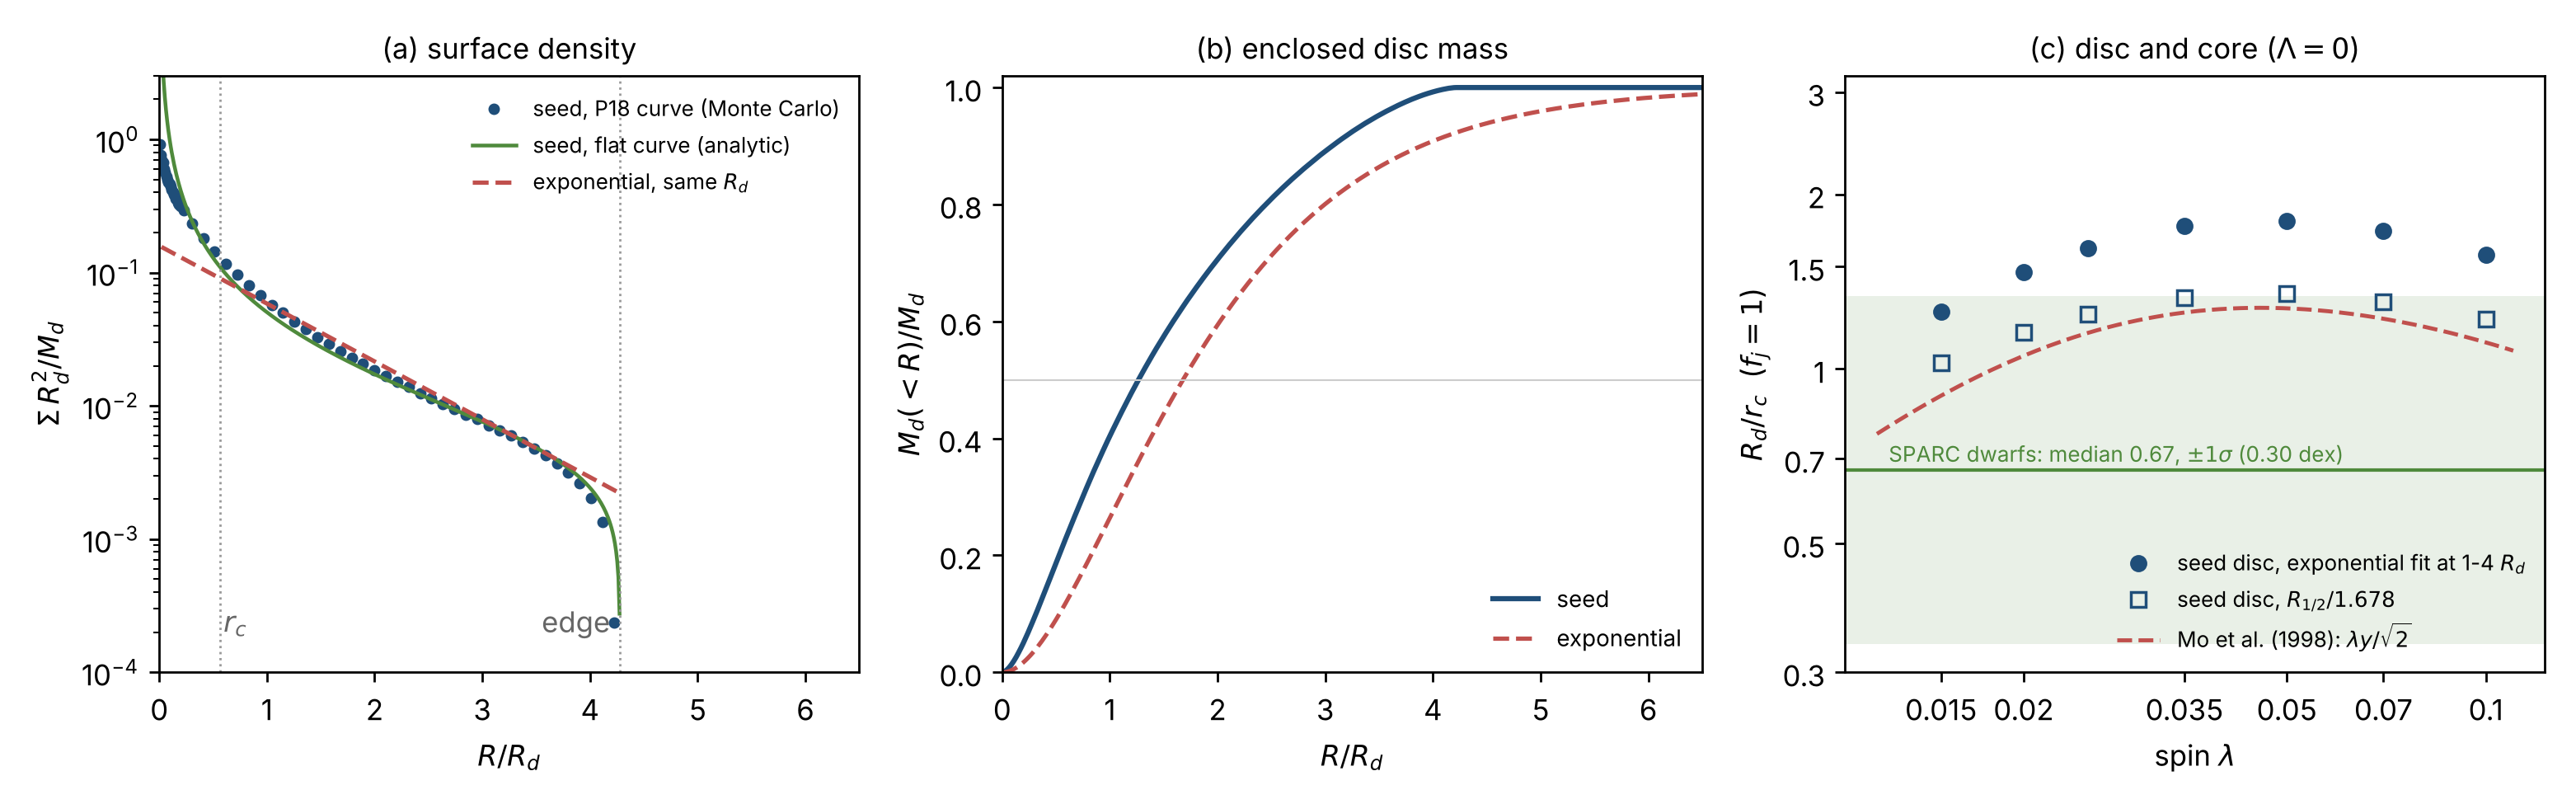
\includegraphics[width=\textwidth]{fig_seed_disc.png}
\caption{The disc made by the seed's own angular momentum ($f_j=1$,
$\Lambda=0$). (a) Surface density for $\lambda=0.035$: Monte Carlo in
the P18 curve (points), the analytic flat-curve result,
Eq.~\eqref{eq:Sigma} (solid), and an exponential disc with the same
scale length (dashed); dotted lines mark the core radius and the edge
$\Rmax$. (b) Enclosed disc mass, seed against exponential. (c) Ratio of
disc scale length to core radius against spin: seed disc with $R_d$ from
an exponential fit at 1--4 $R_d$ (filled) and from the half-mass radius
(open), and the relation of \citet{Mo1998} used in the main paper
(dashed). Green: the median and $1\sigma$ spread of the 79 SPARC dwarfs;
the observed values require $f_j<1$.}
\label{fig:disc}
\end{figure}

For the median spin, $\lambda=0.035$ ($y=50.5$, $\rc=0.020\,\Rb$), the
script gives the following.
\begin{itemize}
\item \emph{Shape.} Between one and four scale lengths the disc is close
  to exponential (Fig.~\ref{fig:disc}a). Inside $0.5\,R_d$ it holds 19\%
  of its mass, twice the 9\% of an exponential disc; the half-mass radius
  is $1.27\,R_d$ instead of $1.68\,R_d$ (Fig.~\ref{fig:disc}b). The disc
  ends at $\Rmax=0.149\,\Rb=4.3\,R_d$.
\item \emph{Effect of the core.} The rising inner curve moves low-$j$
  material outward: inside $S=0.1$ the P18 curve places 15\% of the disc
  mass, the flat curve 23\%. Beyond $S\simeq0.3$ the two agree.
\item \emph{Scale length.} The exponential fit gives
  $R_d=0.035\,\Rb$, $R_d/\rc=1.76f_j$, 1.40 times the Mo--Mao--White
  value $1.26f_j$; the half-mass definition gives $1.33f_j$, 1.06 times
  that value. The difference between the two definitions measures how far
  the seed disc is from exponential.
\item \emph{Dependence on spin.} $R_d/\rc$ changes little with $\lambda$
  (Fig.~\ref{fig:disc}c): $\dd\ln(R_d/\rc)/\dd\ln\lambda=0.16$ at
  $\lambda=0.035$, with a broad maximum near $\lambda\simeq0.05$. The
  reason is the same as in the main paper: a larger spin makes the disc
  larger but also the core larger ($y$ smaller), and the two nearly
  cancel.
\end{itemize}

\section{Relevance to the main paper}

\paragraph{The retained fraction $f_j$.} The observed median
$R_d/\rc=0.67$ is reproduced with a smaller $f_j$ than with the
Mo--Mao--White relation: smaller by the factor 1.06 to 1.4, so the
$f_j\simeq0.77$ of the main paper becomes 0.55--0.73. This is within the
range usually inferred for discs and does not change any conclusion.

\paragraph{The spin test.} The test of the main paper rests on the
\emph{width} of the distribution of $R_d/\rc$. A constant factor does not
change the width, and the weak dependence on $\lambda$ found here (0.16)
is the same as with the Mo--Mao--White relation. The predicted
distribution therefore stays as narrow as before, and the spin test
fails as before.

\paragraph{The shape of real discs.} Detailed conservation of the seed's
angular momentum gives too much mass at the centre and a sharp edge,
the well-known angular-momentum distribution problem of discs that form
by detailed conservation \citep{Dalcanton1997,Bullock2001,vandenBosch2001}.
Late-type dwarfs are bulgeless, so the central excess must have been
removed or redistributed; preferential removal of low-angular-momentum
gas by feedback is the usual explanation
\citep{Governato2010,Brook2011}. The edge near $4.3\,R_d$ is reminiscent
of the truncations and breaks observed in disc profiles at three to five
scale lengths \citep{vanderKruit1979,Pohlen2006}, but a dissipational
disc need not keep the sharp edge of Eq.~\eqref{eq:Sigma}.

\begin{thebibliography}{99}
\bibitem[Brook et al.(2011)]{Brook2011} Brook, C.~B., Governato, F., Ro\v{s}kar, R., et al. 2011, MNRAS, 415, 1051
\bibitem[Bullock et al.(2001)]{Bullock2001} Bullock, J.~S., Dekel, A., Kolatt, T.~S., et al. 2001, ApJ, 555, 240
\bibitem[Dalcanton et al.(1997)]{Dalcanton1997} Dalcanton, J.~J., Spergel, D.~N., \& Summers, F.~J. 1997, ApJ, 482, 659
\bibitem[Fall \& Efstathiou(1980)]{Fall1980} Fall, S.~M., \& Efstathiou, G. 1980, MNRAS, 193, 189
\bibitem[Governato et al.(2010)]{Governato2010} Governato, F., Brook, C., Mayer, L., et al. 2010, Nature, 463, 203
\bibitem[Mestel(1963)]{Mestel1963} Mestel, L. 1963, MNRAS, 126, 553
\bibitem[Mo et al.(1998)]{Mo1998} Mo, H.~J., Mao, S., \& White, S.~D.~M. 1998, MNRAS, 295, 319
\bibitem[Peebles(1969)]{Peebles1969} Peebles, P.~J.~E. 1969, ApJ, 155, 393
\bibitem[Pohlen \& Trujillo(2006)]{Pohlen2006} Pohlen, M., \& Trujillo, I. 2006, A\&A, 454, 759
\bibitem[van den Bosch et al.(2001)]{vandenBosch2001} van den Bosch, F.~C., Burkert, A., \& Swaters, R.~A. 2001, MNRAS, 326, 1205
\bibitem[van der Kruit(1979)]{vanderKruit1979} van der Kruit, P.~C. 1979, A\&AS, 38, 15
\end{thebibliography}

\appendix
\section{Code}\label{app:code}
\lstinputlisting{code/seed_disc.py}

\noindent Output (\texttt{code/seed\_disc\_output.txt}):
\lstinputlisting[language={}]{code/seed_disc_output.txt}

\end{document}
